\chapter{Generator}
\label{chap:Generator}

There are number solutions that provide formulas in a way of generators or benchmarks:

\begin{itemize}
  \item SMT-LIB \cite{BarFT-RR-17} -- is project aimed at facilitating research and development in \gls{SMT} . One part of their activity is defining syntax for representing formulas in with various theories and hosting considerable benchmark library
  \item SATLIB \cite{Hol00} -- is collection of benchmarks of propositional logic (DIMACS CNF format)
  \item Tough SAT \cite{ToughSAT} -- is a platform that will generate boolean CNF formulas that encode "difficult" problems. Problems are represented in propositional logic (DIMACS CNF format). Although Tough SAT is in fact generator it supports only several predefined problems like Factoring, Subset Sum, Random k-SAT, Cocktail.
% \item PySAT\footnote{\url{https://pysathq.github.io/}} -- is a toolkit, which aims at providing a simple and unified interface to a number of SAT solvers as well as to a variety pseudo-Boolean encodings. Rather than generating benchmarks this tool is useful when there is a need to access several solvers with unified interface.
  \item CNFgen \cite{CNFGen} -- produces combinatorial benchmarks in DIMACS format. These benchmarks come mostly from research in Proof Complexity (pigeonhole principle, ordering principle, k-clique and more). Many of these formulas encode structured combinatorial problems well known to be challenging for certain SAT solvers.
  \item \gls{TSTP} (Thousands of Solutions from Theorem Provers) a side project of \gls{TPTP} \cite{Sut17} -- it is a library of problems and solutions encoded in TPTP format
\end{itemize}

Although a lot of ready to use benchmarks can be found, there are not a lot of generators. Tough SAT and CNFgen are generators that generate predefined problem with given size, SMT-LIB, SATLIB, TSTP are mainly repositories of benchmarks, not generators itself. Out of mentioned solutions only SMT-LIB and TSTP support first order logic. None of mentioned solutions can generate first order logic formulas. 

A random first order formula would be useful in this sense, that it would allow creating new datasets with precisely controlled elements. A parameters for such generator shall be described next.

\newpage

\section{Defining CNF Generator}

User defines generator in 2 steps:

\begin{enumerate}
  \item General setting for generated formula

    In this step user defines set of allowed \gls{FOL} elements:
    \begin{itemize}
      \item set of variable names $\{'v1','v2',\dots\}$
      \item set of functor names $\{'f1','f2',\dots\}$
      \item set of predicate names $\{'p1','p2',\dots\}$
      \item set of allowed functor arities $a_f = \{0, 1, 2,\dots\}$
      \item maximum recursion depth $n$ for functors
      \item set of allowed predicate arities $a_p = \{0, 1, 2,\dots\}$
      \item set of atom allowed connectives, that is no connective or/and any subset of $AllowedConnectives = \{=, !=, \emptyset\}$
      \item set of allowed clause lengths $AllowedClausesLengths = \{1,2,\dots\}$
      \item amount of literals to be negated
    \end{itemize}

  \item How many instances of elements are allowed

    In this step user defines what properties formula should have:
    \begin{itemize}
      \item formula contains from $c_{min}$ to $c_{max}$ clauses
      \item formula contains from $l_{min}$ to $l_{max}$ literals
    \end{itemize}
\end{enumerate}

Basic algorithm of generating formula consists of following steps:

\begin{enumerate}
  \item Resolve user constraints~\ref{sec:ResolveUserConstrains}
  \item Generate possible formula based on generators~\ref{sec:Generators}
  \item Generate statistics and export formula to file~\ref{sec:GenerateStatisticsAboutFormula}
\end{enumerate}


\section{Resolve user constraints}
\label{sec:ResolveUserConstrains}

User constrains are defined in input parameters as $AllowedClausesLengths$, $NumberOfClauses$, $NumberOfLiterals$. To generate random formula withing these constrains, number of clauses with appropriate clause length must be computed.

CNF formula $F_{cnf}$ consists of unordered clauses $c1, c2, \dots$. 

\begin{align*}
	&F_{cnf}(x) = \{c1, c2, \dots\, cx\} \\
	\text{where }
		&x \text{ -- number of clauses in formula}
\end{align*}

If we group clauses by their length:
\begin{align*}
	&F_{cnf}(x) = \bigcup_{i=1}^c c_i \\
	\text{where }
		&c_i \text{ -- set of clauses with length i} 
\end{align*}

Number of literals in formula can be represented as:
\begin{align*}
	l(x) &= x_1|c_1| + x_2|c_2| + \dots + x_x|c_x| = \sum_{i=1}^{x} x_i |c_i| \\
	x &= x_1 + x_2 + \dots + x_n \\
	c_i &\in AllowedClausesLen: \forall_{i \neq j} c_i \neq c_j  \\
	\text{where }
		&x \text{ -- number of clauses in formula} \\ 
		&l(x) \text{ -- number of literals in formula} \\ 
		&|c_i| \text{ -- number of clauses with length i} 
\end{align*}

So in the end:

\begin{align}
  l(x) &= \sum_{i=1}^{x} x_i |c_i|\label{eq:UserConstraintsLx} \\
  x &= \sum_i^x x_i\label{eq:UserConstraintsX} \\
  l_{min} &< l(x) < l_{max} \label{eq:UserConstraintsRangeL}\\
  c_{min} &< x < c_{max}\label{eq:UserConstraintsRangeC} \\
	\text{where } 
		&x \text{ -- number of clauses in formula} \nonumber \\
		&l(x) \text{ -- number of literals in formula} \nonumber  \\
		&|c_i| \text{ -- number of clauses with length i} \nonumber
\end{align}

Solution of above equation are pairs of numbers: clause length and how many clauses with this length should be used in generated clause.

\subsection{Using Z3 to resolve user constraints}

Z3 \cite{Z3Solver} is a \gls{SMT} prover from Microsoft Research. It uses SMT-LIB as input format, but also has bindings to multiple languages. It can be used to solve user constraints presented in~\ref{sec:ResolveUserConstrains}. Z3 supports arithmetic what is essential for solving user constraints.

Solving equation is implemented as class $CNFConstraintSolver$ (picture~\ref{pic:ConstraintSolverZ3ClassDiagram}). Parameter $allowed\_clause\_lengths$ corresponds to $c_i$ in equation~\ref{eq:UserConstraintsLx}, parameter $number\_of\_literals$ corresponds range of allowed values of literals - tuple of minimal and maximum range - ($l(x)$ in equation~\ref{eq:UserConstraintsLx}), parameter $number\_of\_clauses$ corresponds number of allowed values of clause - tuple of minimal and maximum range - ($x$ in equation~\ref{eq:UserConstraintsX}). The set of variables $x_i$ will be returned from method $solve()$ as dictionary, where key is $i$ (clause length) and value is how many clauses are needed.


\begin{figure}[h]
\begin{centering}
  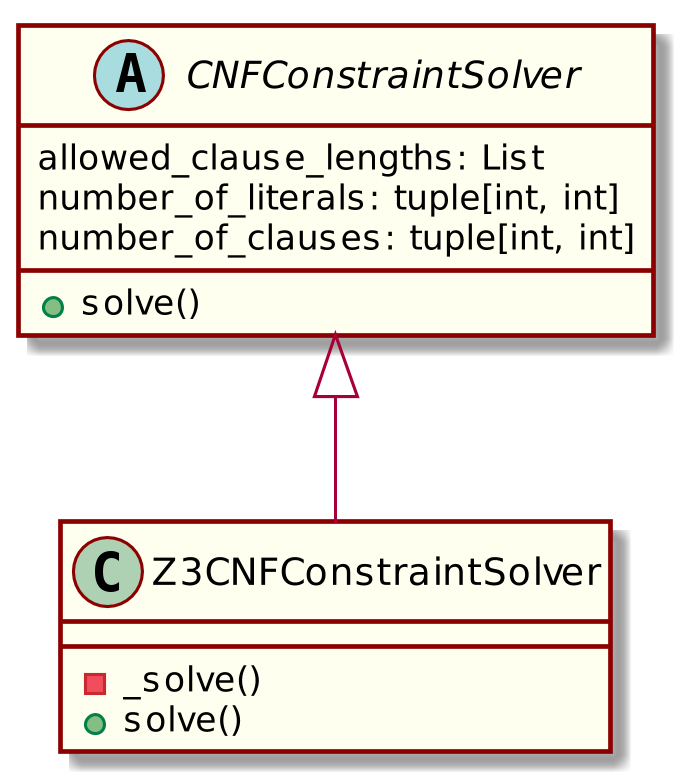
\includegraphics[width=0.3\textwidth]{logic-formula-generator/fol/resolve_constraints.png}
  \caption{Subclassed constraint solver}
  \label{pic:ConstraintSolverZ3ClassDiagram}
\end{centering}
\end{figure}

Function \mintinline{text}{_solve()} in listing \ref{lis:DeterministicSolve} solves user constraints using Z3 solver bindings in Python. Line 
\mintinline{python}{X = [z3.Int() ...]}
defines Z3 variables, which can contain only integer values. This variable is used to represent $x_i$ from \ref{eq:UserConstraintsX}. Further down the line 
\mintinline{python}{s = z3.Solver()} 
creates model, to which constraints will be added. Constraints are defined by functions
\mintinline{python}{z3.Sum}, 
\mintinline{python}{z3.And}, 
and can be added to model via
\mintinline{python}{s.add}.
Variables must follow 2 rules: they must be non negative and be in range defined by \ref{eq:UserConstraintsRangeC} and \ref{eq:UserConstraintsRangeL}. Solution can be calculated from model with 2 operations: first check if model is satisfayable, next evalueate (get value) of variables in model. If another solution is needed, it can be done by adding constraints, that forbids concurrencyent solution and recalculating model.


\begin{listing}[H]
  \caption{Lazy, deterministic function for solving user constraints}
  \label{lis:DeterministicSolve}
\begin{minted}{python}
    def _solve(self) -> Iterable[Dict[int, int]]:
        """Solve in deterministic order"""
        A = self.literal_coefficients
        n = len(A)
        X = [z3.Int() for i in range(n)]
        s = z3.Solver()

        # solutions must be positive
        s.add(z3.And([X[i] >= 0 for i in range(n)]))

        # clauses must be in range
        s.add(z3.Sum(X) <= self.number_of_clauses[1])
        s.add(z3.Sum(X) >= self.number_of_clauses[0])

        # literals must be in range
        s.add(z3.Sum([A[j] * X[j] for j in range(n)]) <= self.number_of_literals[1])
        s.add(z3.Sum([A[j] * X[j] for j in range(n)]) >= self.number_of_literals[0])

        while s.check() == z3.sat:
            solution = [s.model().evaluate(X[i]) for i in range(n)]
            yield {clause_len: s.as_long() for clause_len, s in zip(A, solution)}
            forbid = z3.Or([X[i] != solution[i] for i in range(n)])
            s.add(forbid)
\end{minted}
\end{listing}

Fundamental problem of using SAT (or SMT) solver in this scenario when any, random solution is needed, is fact that solver will always produce deterministic result for the same input data. There are 2 solutions for this problem. First one, presented here, is using a wrapper that will temporarily skip or discard part of solutions, to randomize deterministic output. In this cave, non public function $\_solve$ in listing~\ref{lis:DeterministicSolve} is a function that actually yields solutions and $solve$ in listing \ref{lis:RandomSolve} is a randomizing wrapper. Randomization occurs at the cost of time and memory. Second approach assumes that solver supports soft clause\footnote{contrary to hard clauses, soft clauses does not have to be satisfied}. Using soft clauses a random starting point can be suggested to a solver. For example line added to listing \ref{lis:DeterministicSolve} \mintinline{python}{s.add(z3.Sum([A[j] * X[j] for j in range(n)]) == random_number))} would hint Z3 solver to strat in \mintinline{text}{random_number} if Z3 supported this feature in Python bindings.

\begin{listing}[H]
  \caption{Lazy, randomizing wrapper around deterministic solver~\ref{lis:DeterministicSolve}}
  \label{lis:RandomSolve}
\begin{minted}{python}
    def solve(self, skip_chance: float = None):
        """Solve in random order"""
        skip_chance = random.random() if skip_chance is None else skip_chance
        cache = []
        for solution in self.solve():
            if random.random() < skip_chance:
                yield solution
            else:
                cache.append(solution)

        random.shuffle(cache)
        for cached_solution in cache:
            yield cached_solution
\end{minted}
\end{listing}

\section{Intermediate representation}

Abstract syntax tree of \gls{FOL} is implemented in the same way as mathematical definition, see picture~\ref{pic:fol_elements_class_diagram}. All classes have base class $FolElement$ so that they can be easily identified as element of first order logic and introduce visitor pattern. Visitor pattern is used for exporting formula from intermediate representation to the format of choice (like \gls{TPTP}) as well as counting statistics about generated formula. See for example listing~\ref{lis:TPTPExample} - it is convention from TPTP to store some statistics about file at the beginning of file as comment.

Variable and functor are terms, that is why the inherit from term class. Functor is recursive structure it can contain variable or another term, that is why it is connected with aggregation with term class. Predicate can contain only terms, atom can contain term or predicate, literal can contain only one atom but adds sign to it, clause is one or more literal, CNF formula is one or more clause.

\begin{figure}[h]
\begin{centering}
  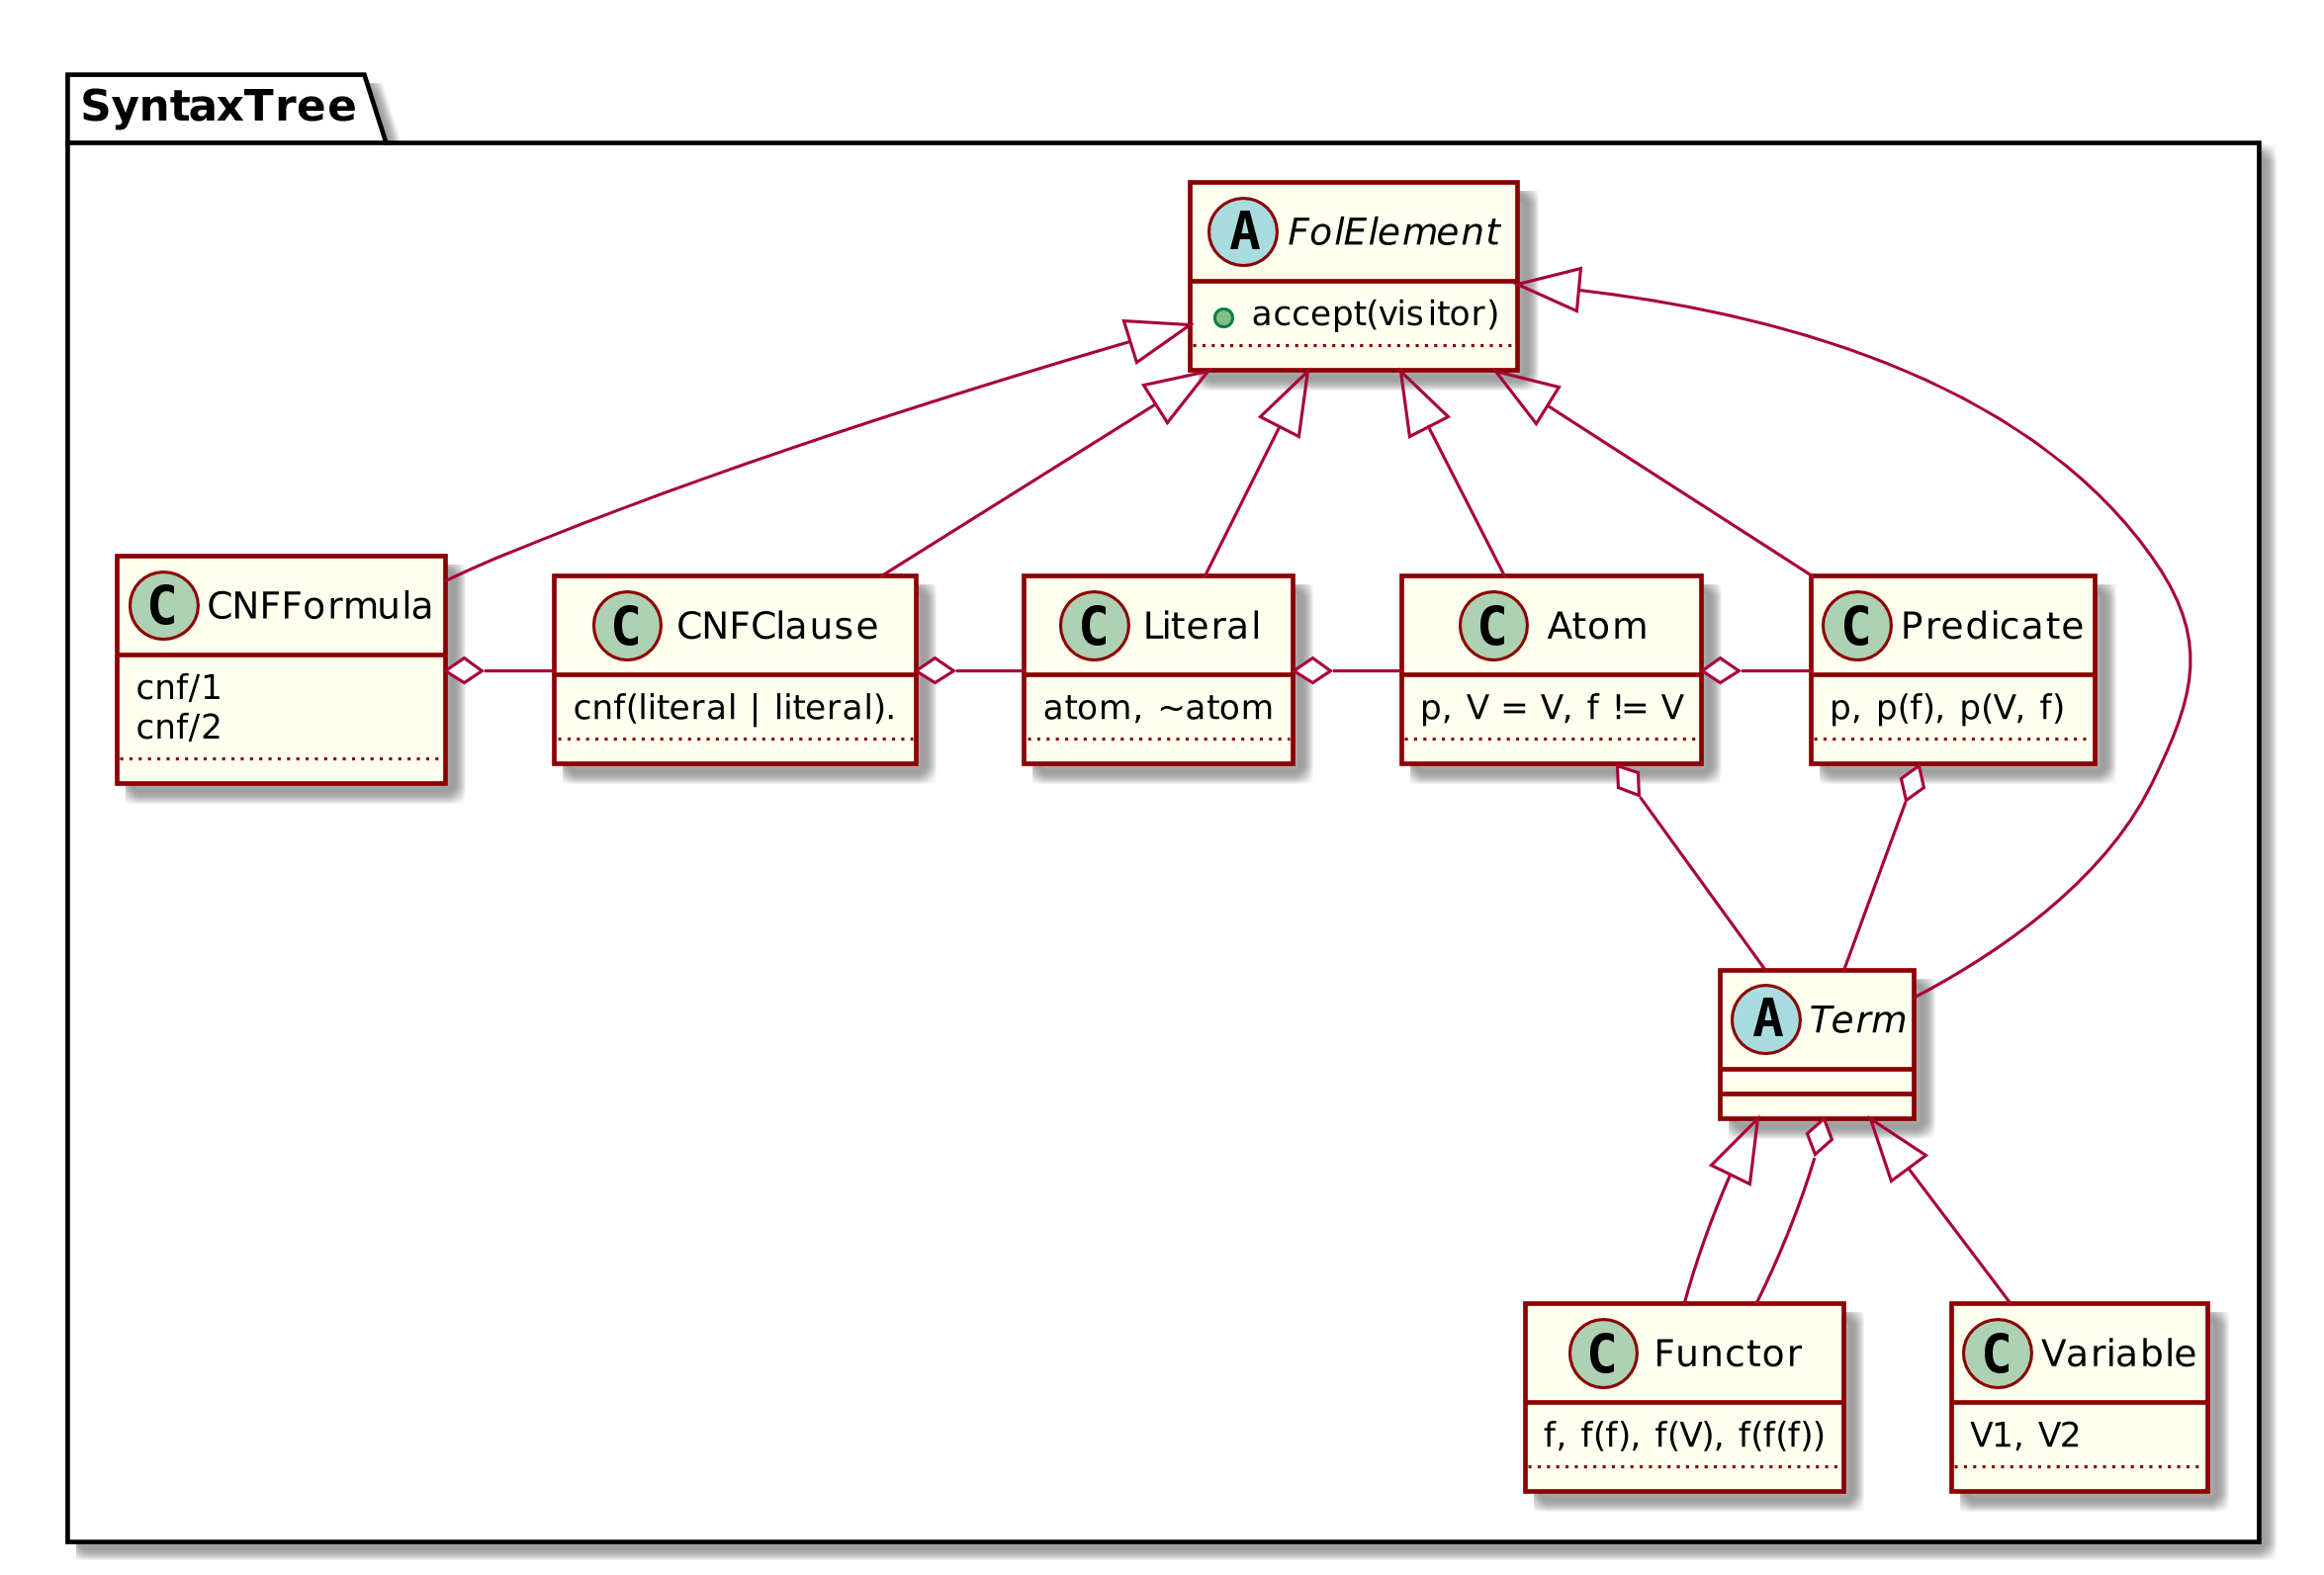
\includegraphics[width=\textwidth]{logic-formula-generator/fol/cnf_fol_elements.png}
  \caption{Class diagram for internal representation of first order logic elements}
  \label{pic:fol_elements_class_diagram}
\end{centering}
\end{figure}

\section{Intermediate representation generators}
\label{sec:Generators}

Generators are implemented as cascade (picture~\ref{pic:fol_signature_generator_class_diagram}), that is formula generator provides formulas, but requires clause generator, clause generator provides clauses, but requires literal generator and so on.

\begin{figure}[h]
\begin{centering}
  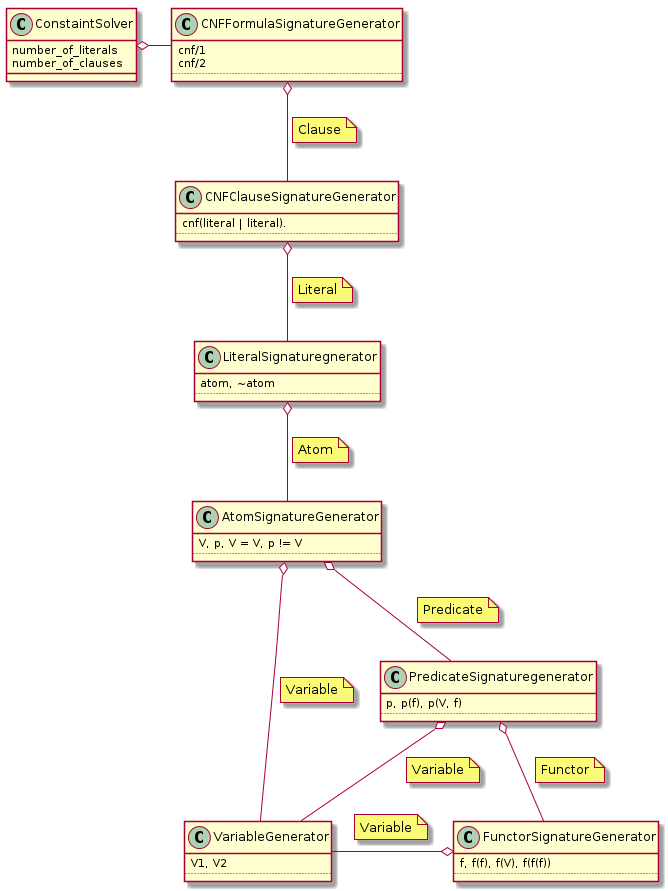
\includegraphics[width=0.7\textwidth]{logic-formula-generator/fol/cnf_signature_generators.png}
  \caption{Class diagram of generators in CNF formula generator}
  \label{pic:fol_signature_generator_class_diagram}
\end{centering}
\end{figure}

Manual creation of generators is required only in advanced case. To automate this process $CNFFormulaGenerator$ (picture~\ref{pic:cnf_generator_class_diagram}) has been created. This is interface for user to create random CNF formulas that will automatically resolve user constraints and yield random formula. After creating formula from signature generators formula will be post processed - given random names and optionally negation sign. Generated formula can be then exported to file along with statistics about formula.

\begin{figure}[h]
\begin{centering}
  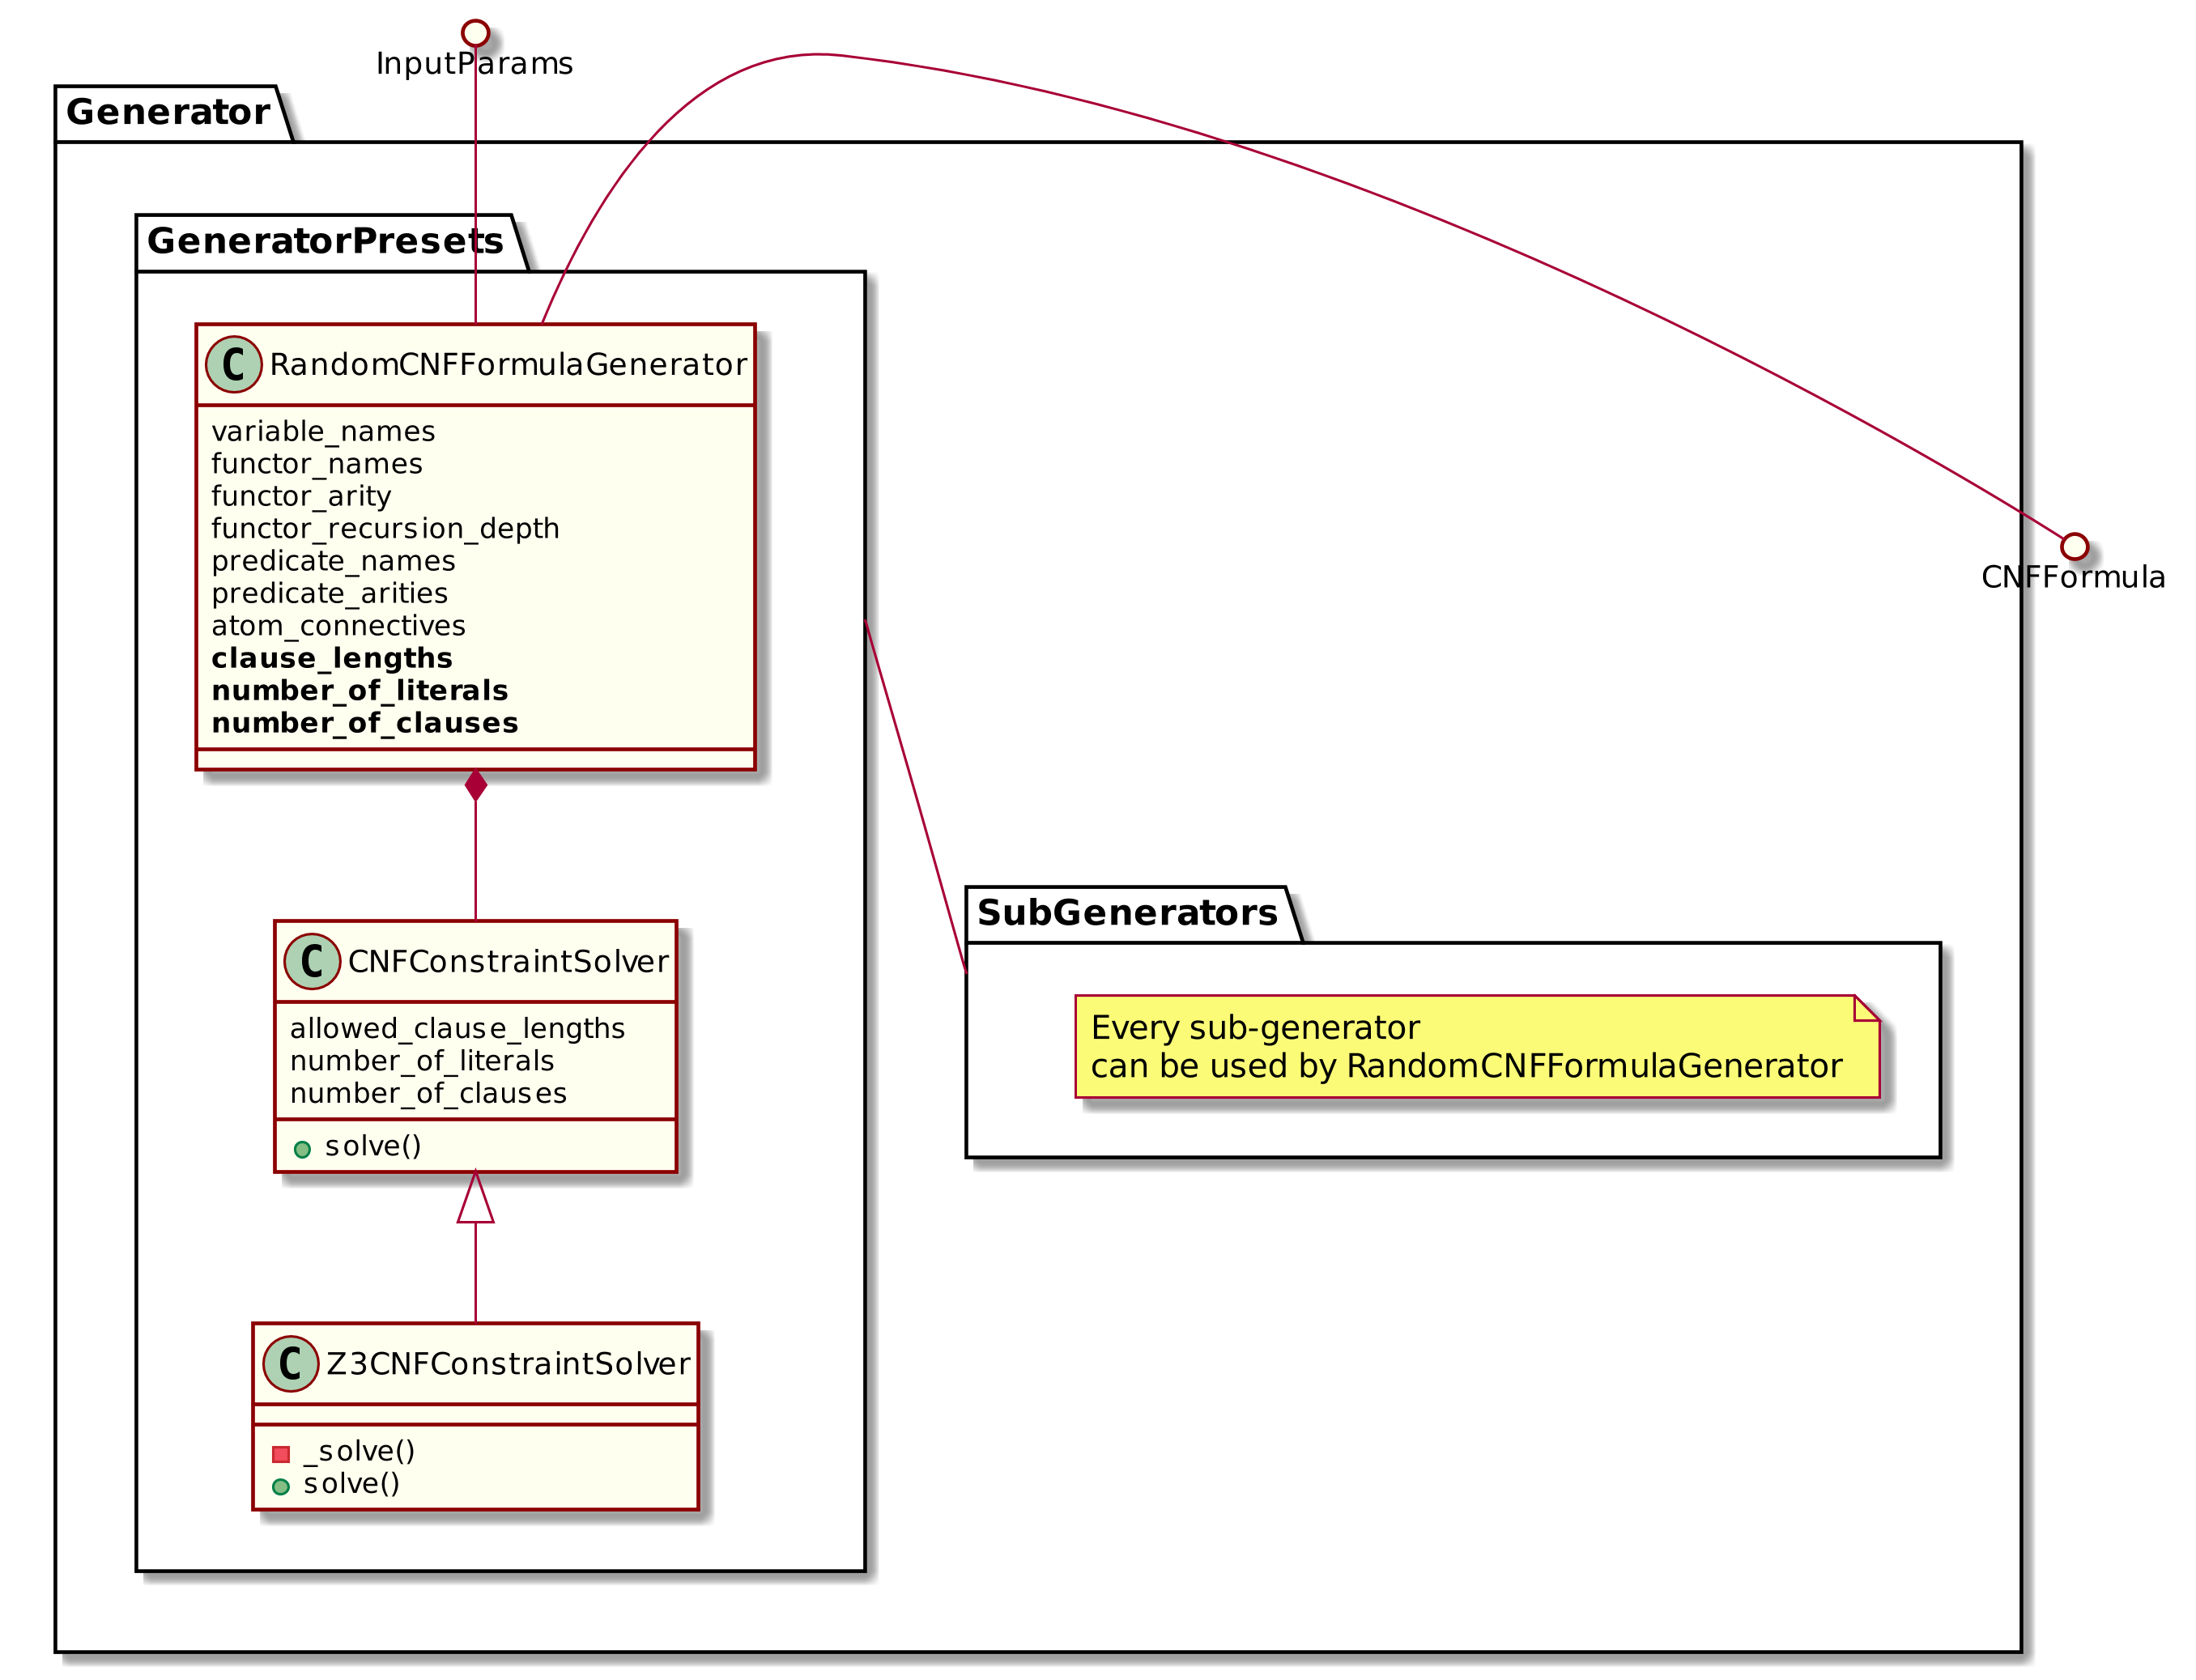
\includegraphics[width=\textwidth]{logic-formula-generator/cnf_formula_generator.png}
  \caption{Class diagram of CNF formula generator}
  \label{pic:cnf_generator_class_diagram}
\end{centering}
\end{figure}

\section{Export and generate statistics about formula}
\label{sec:GenerateStatisticsAboutFormula}

After generating formula it would be usefull to gather some information about it. 

\begin{figure}[h]
\begin{centering}
  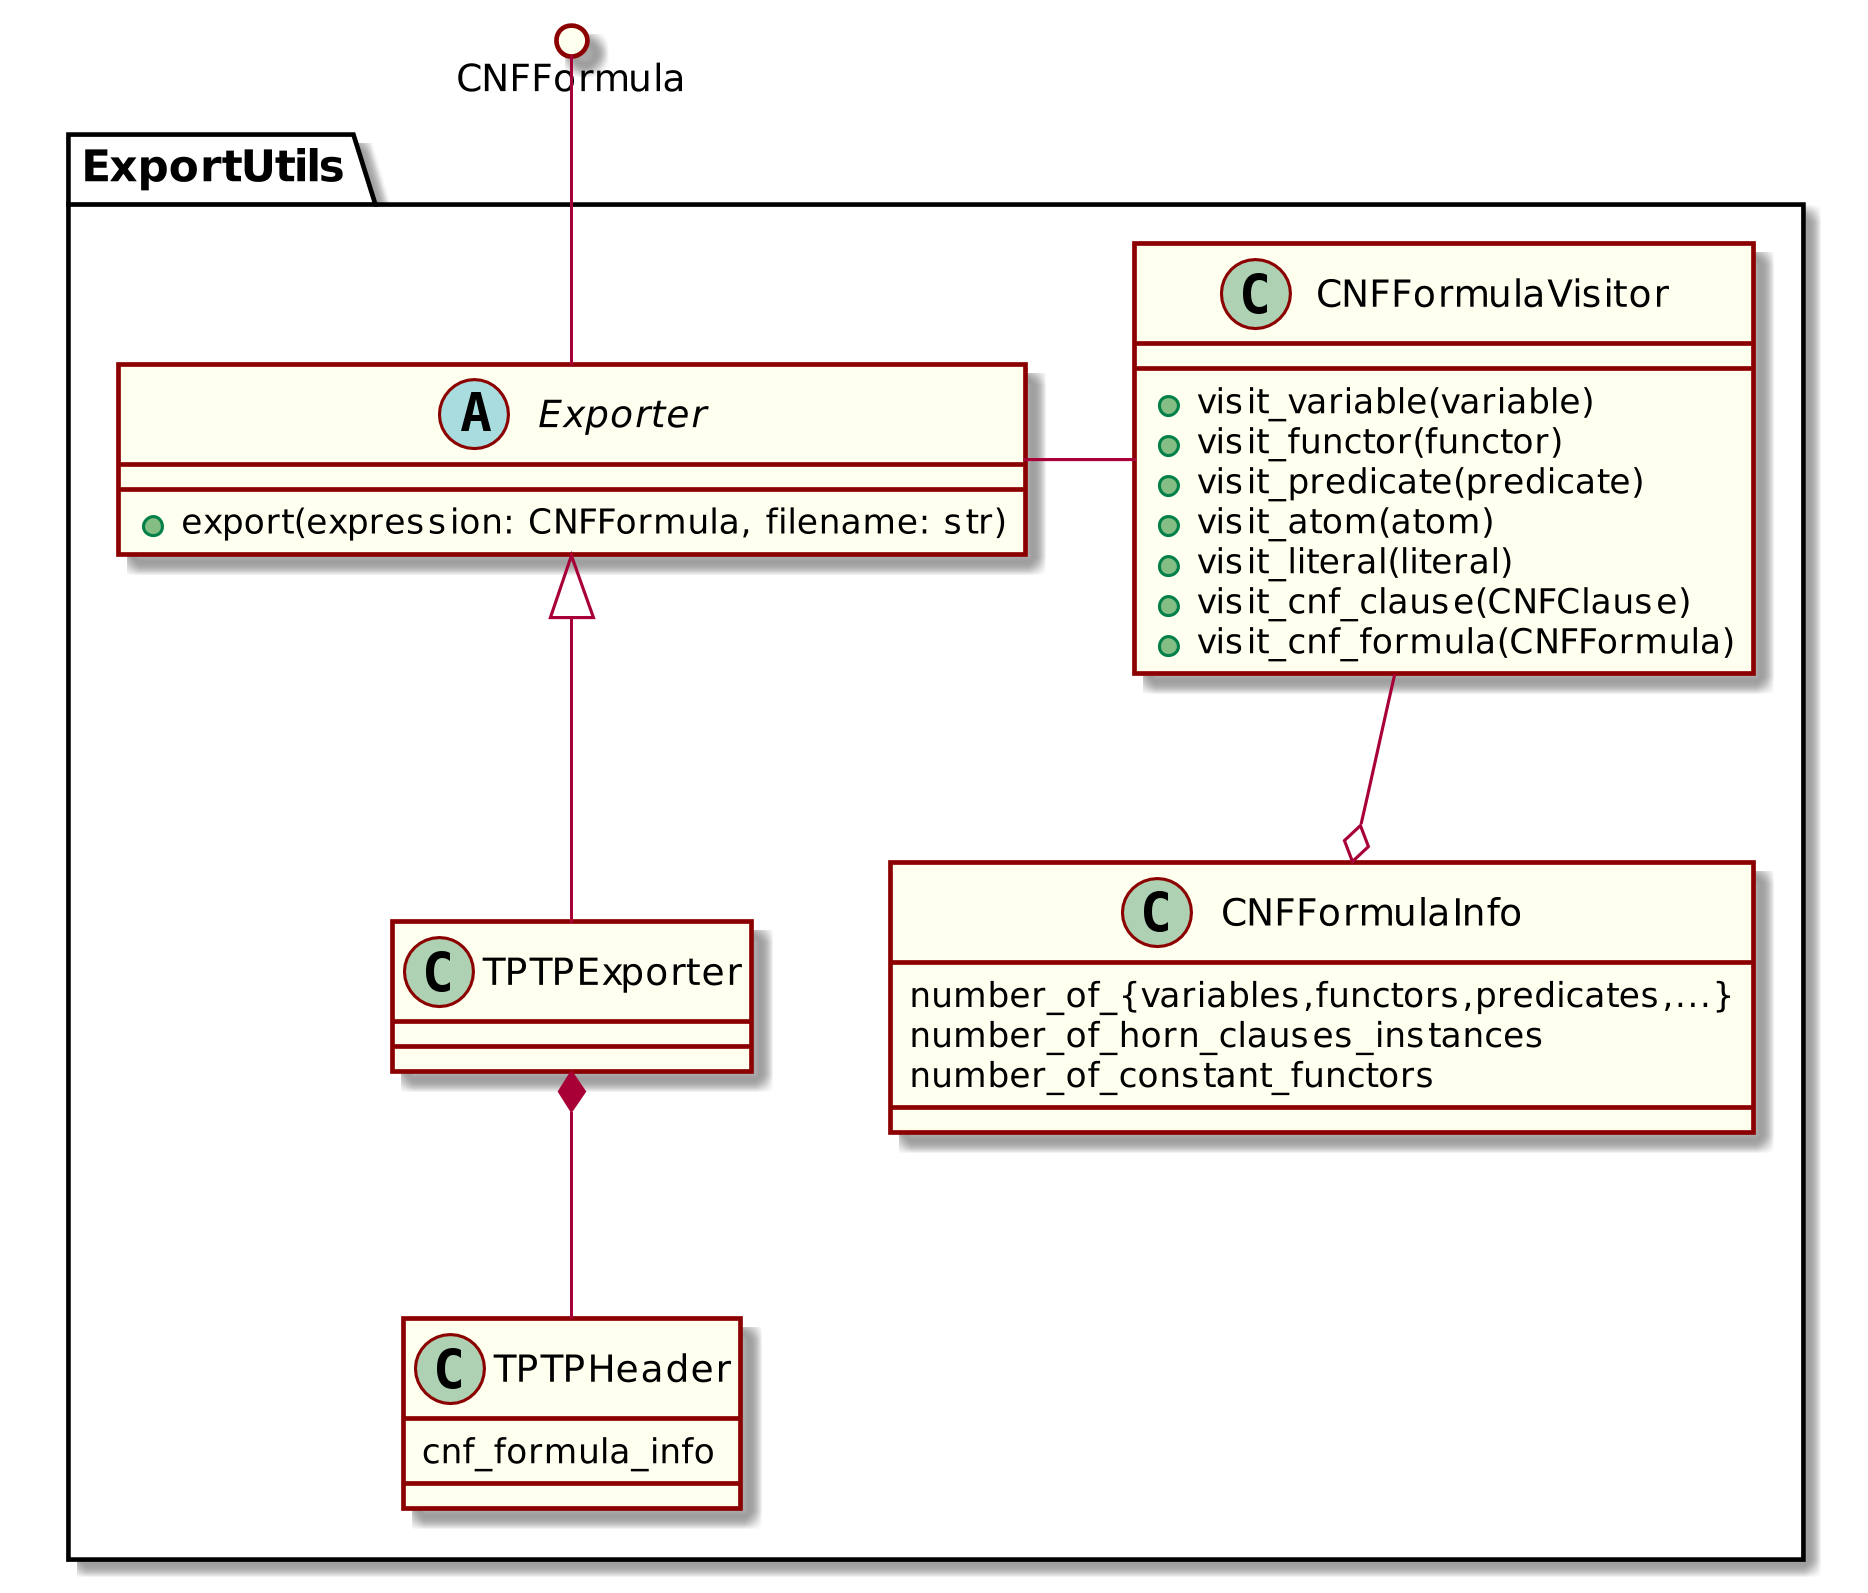
\includegraphics[width=\textwidth]{logic-formula-generator/fol/cnf_formula_statistics.png}
  \caption{Classes for which take part in generating statistics and exporting FOL CNF formula}
  \label{pic:CNFFormulaInfo}
\end{centering}
\end{figure}
